\begin{figure*}
    \centering
    \begin{subfigure}{0.3\textwidth}
        \centering
        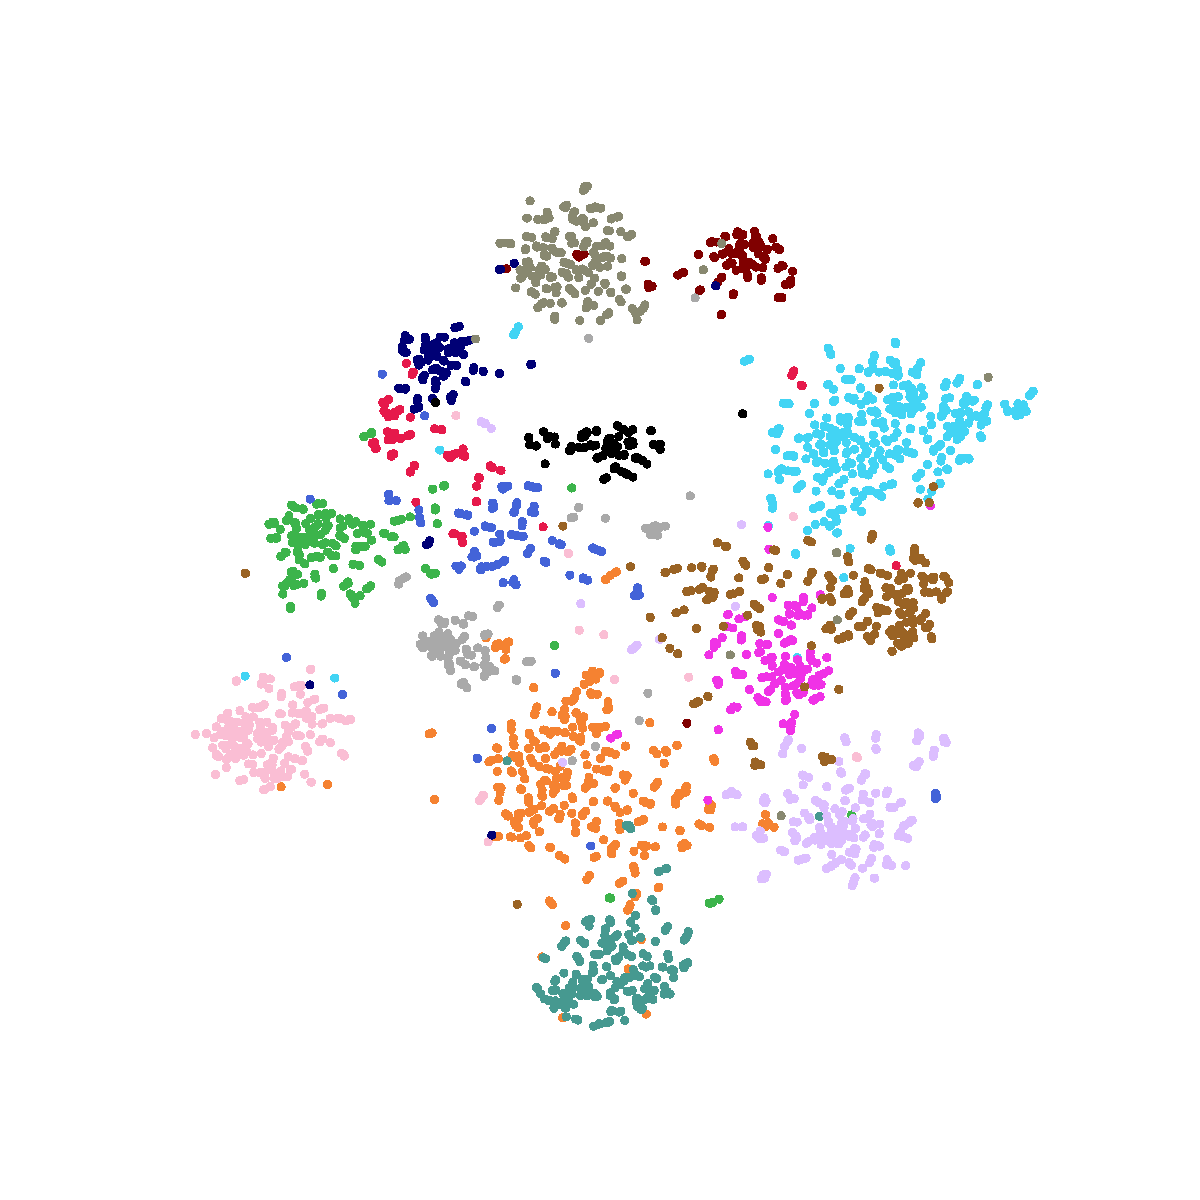
\includegraphics[width=\linewidth]{fig/tsne/point_mae1.pdf}
        \caption*{\textbf{\#TP}:22.1M \textbf{\#OA}:85.18}
        \caption{Full fine-tuning}
        \label{fig:sub1}
    \end{subfigure}
    \hfill
    \begin{subfigure}{0.3\textwidth}
        \centering
        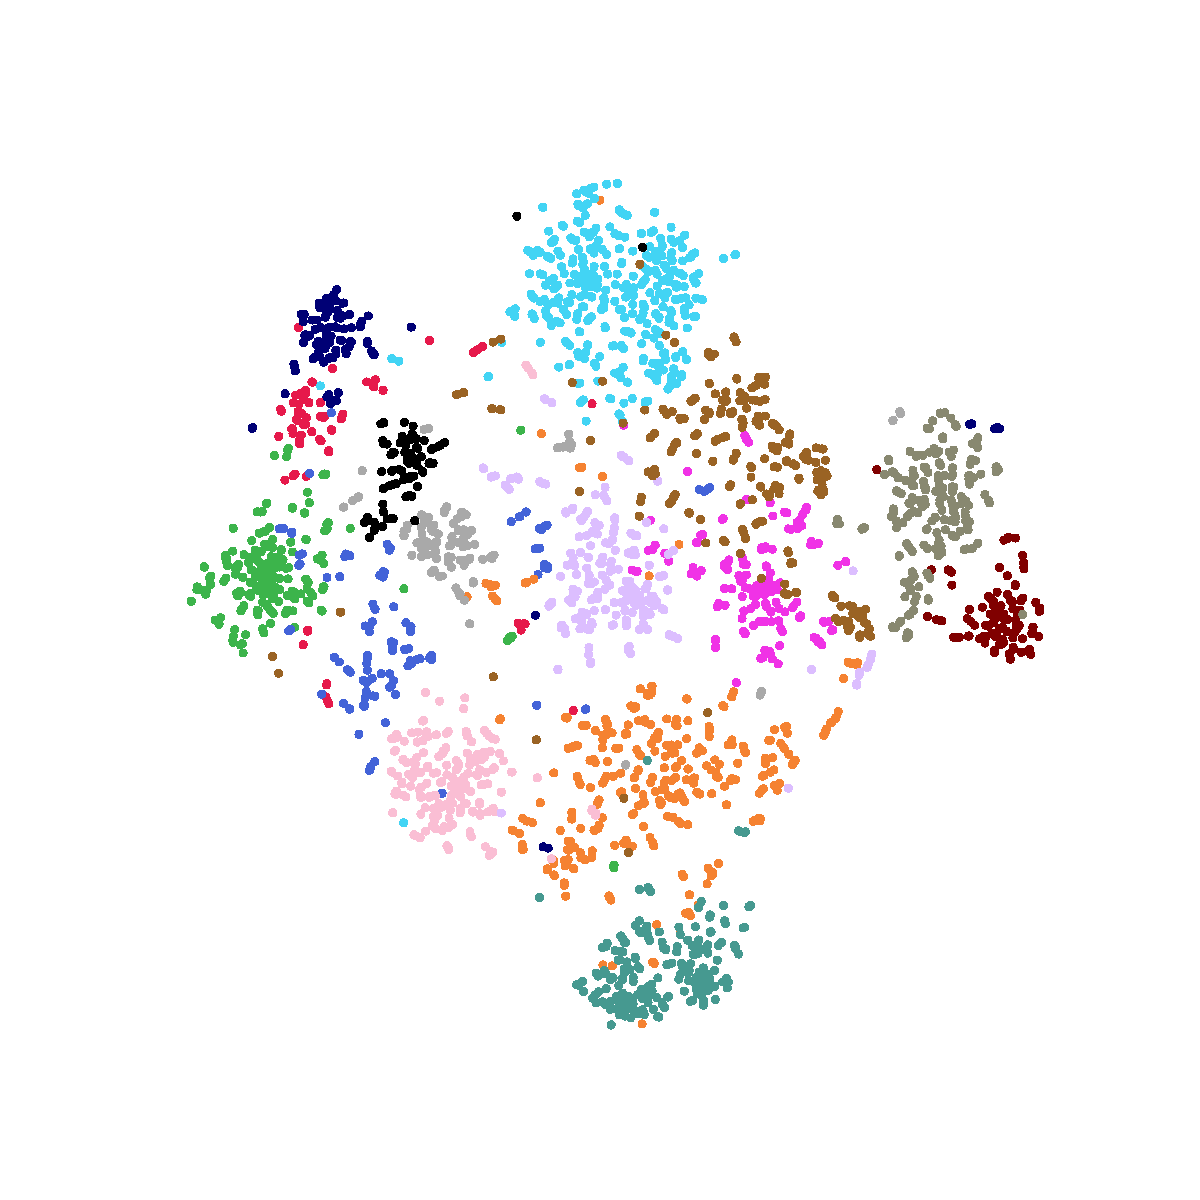
\includegraphics[width=\linewidth]{fig/tsne/idpt1.pdf}
        \caption*{\textbf{\#TP}:1.7M \textbf{\#OA}:84.94}
        \caption{IDPT}
        \label{fig:sub2}
    \end{subfigure}
    \hfill
    \begin{subfigure}{0.3\textwidth}
        \centering
        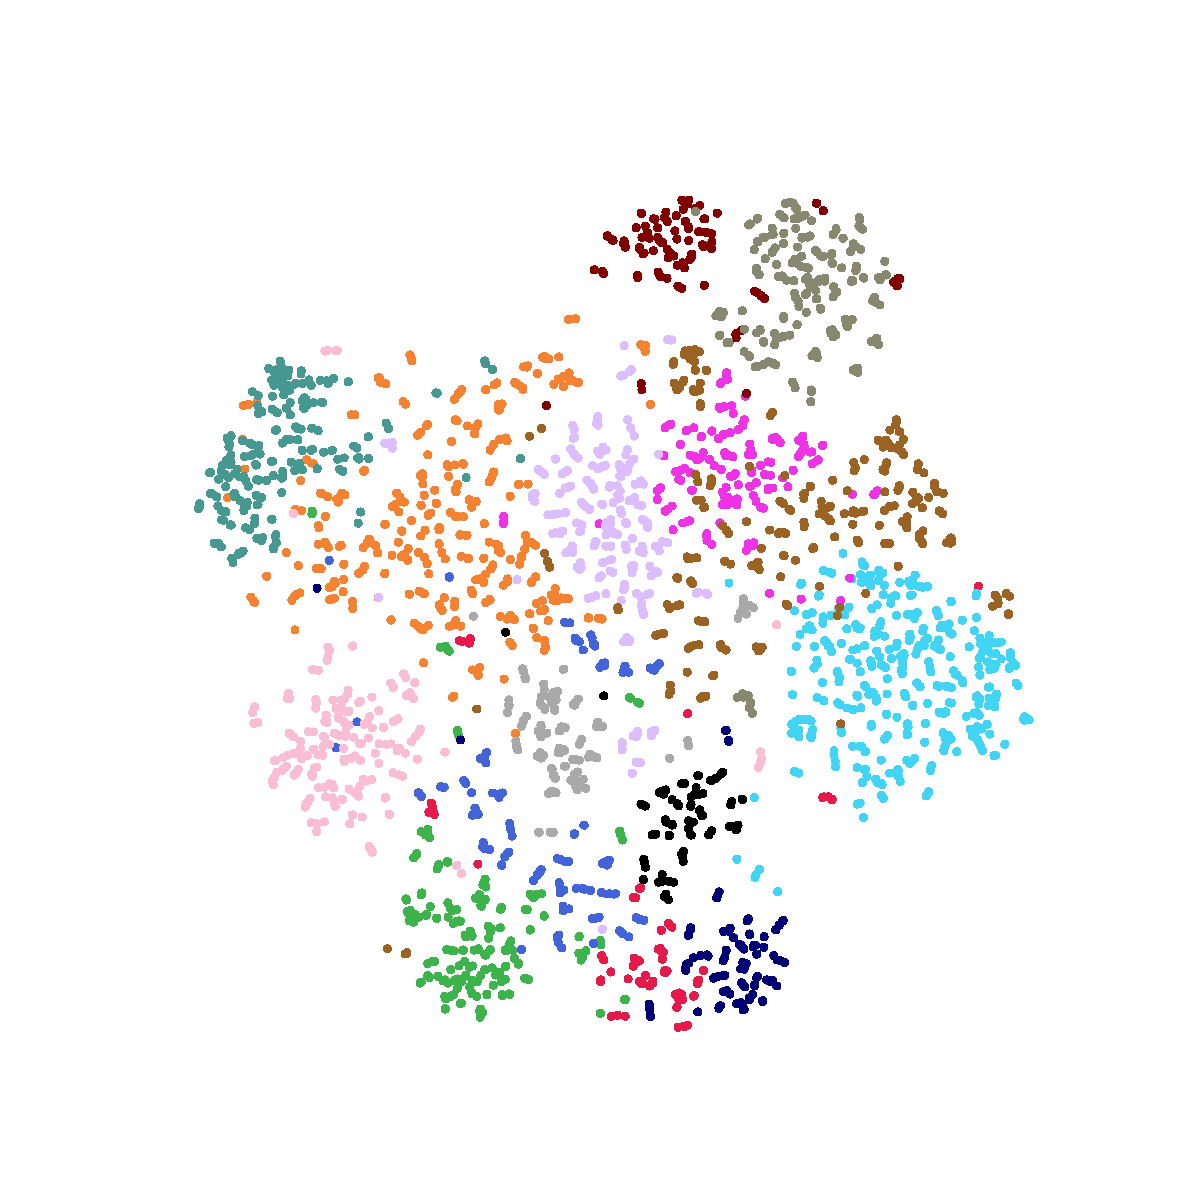
\includegraphics[width=\linewidth]{fig/tsne/dapt1.pdf}
        \caption*{\textbf{\#TP}:1.1M \textbf{\#OA}:85.08}
        \caption{DAPT}
        \label{fig:sub3}
    \end{subfigure}
    \hfill
    \begin{subfigure}{0.3\textwidth}
        \centering
        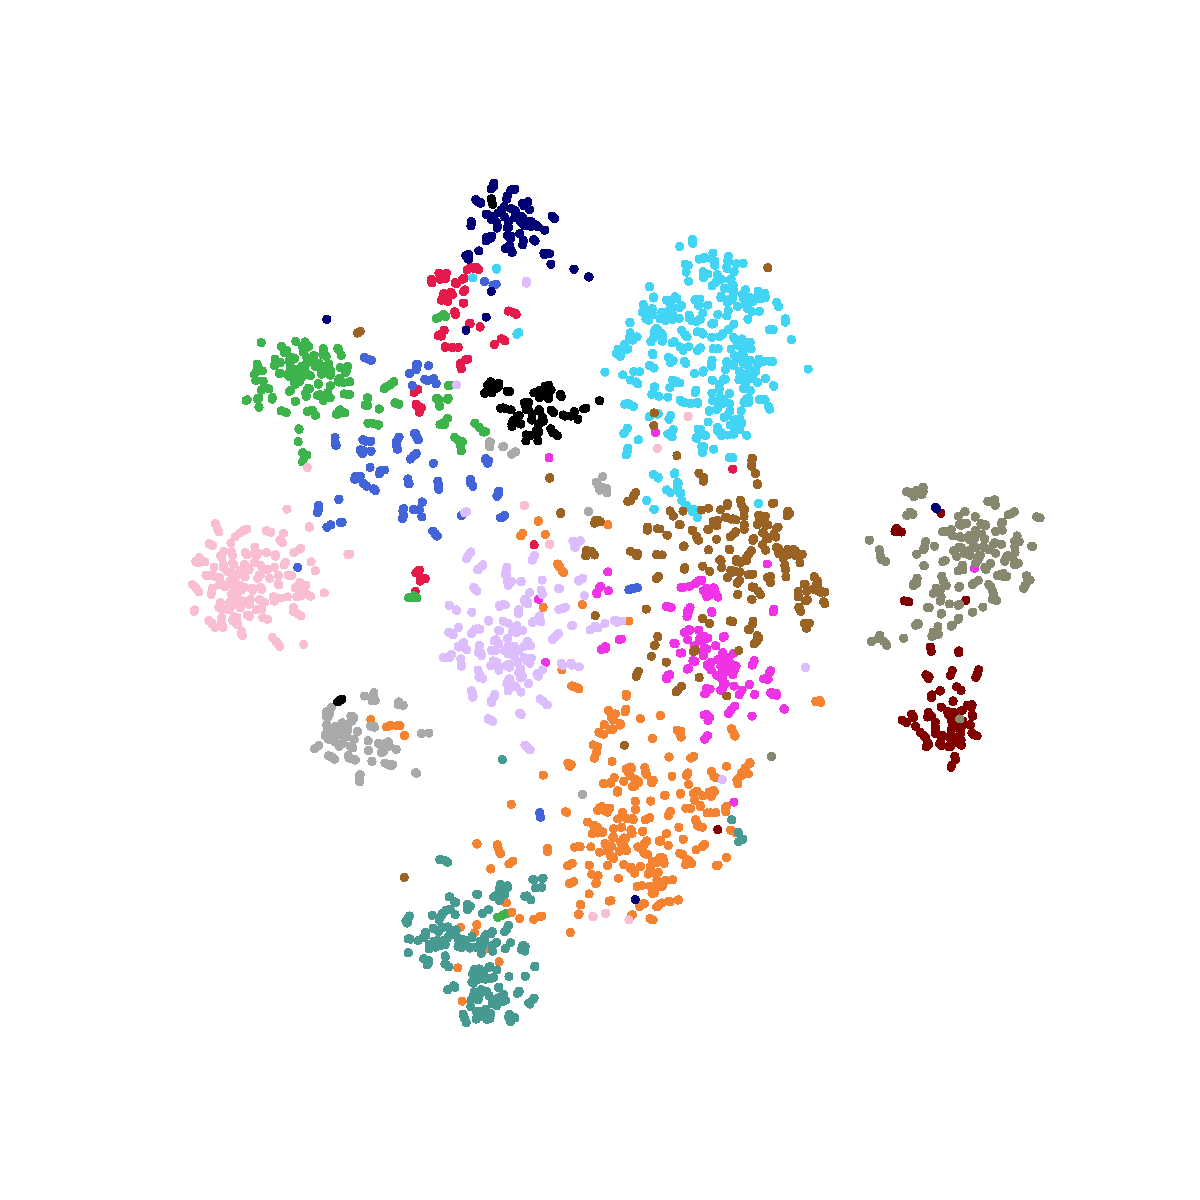
\includegraphics[width=\linewidth]{fig/tsne/PPT1.pdf}
        \caption*{\textbf{\#TP}:1.1M \textbf{\#OA}:84.91}
        \caption{PPT}
        \label{fig:sub4}
    \end{subfigure}
    \hfill
    \begin{subfigure}{0.3\textwidth}
        \centering
        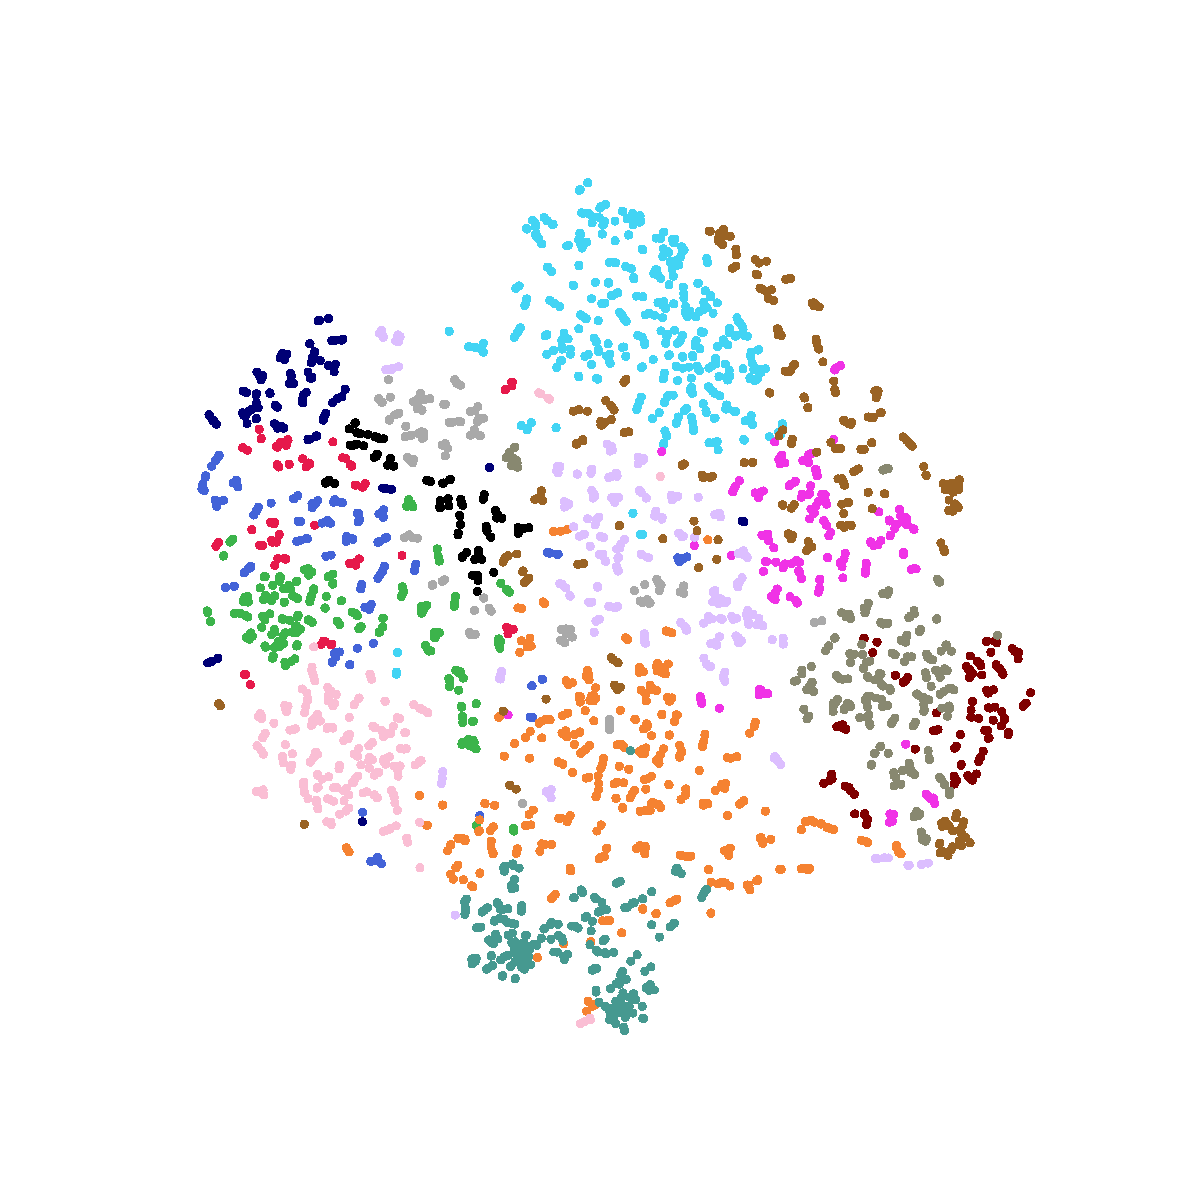
\includegraphics[width=\linewidth]{fig/tsne/LST1.pdf}
        \caption*{\textbf{\#TP}:0.8M \textbf{\#OA}:82.75}
        \caption{LST}
        \label{fig:sub5}
    \end{subfigure}
    \hfill
    \begin{subfigure}{0.3\textwidth}
        \centering
        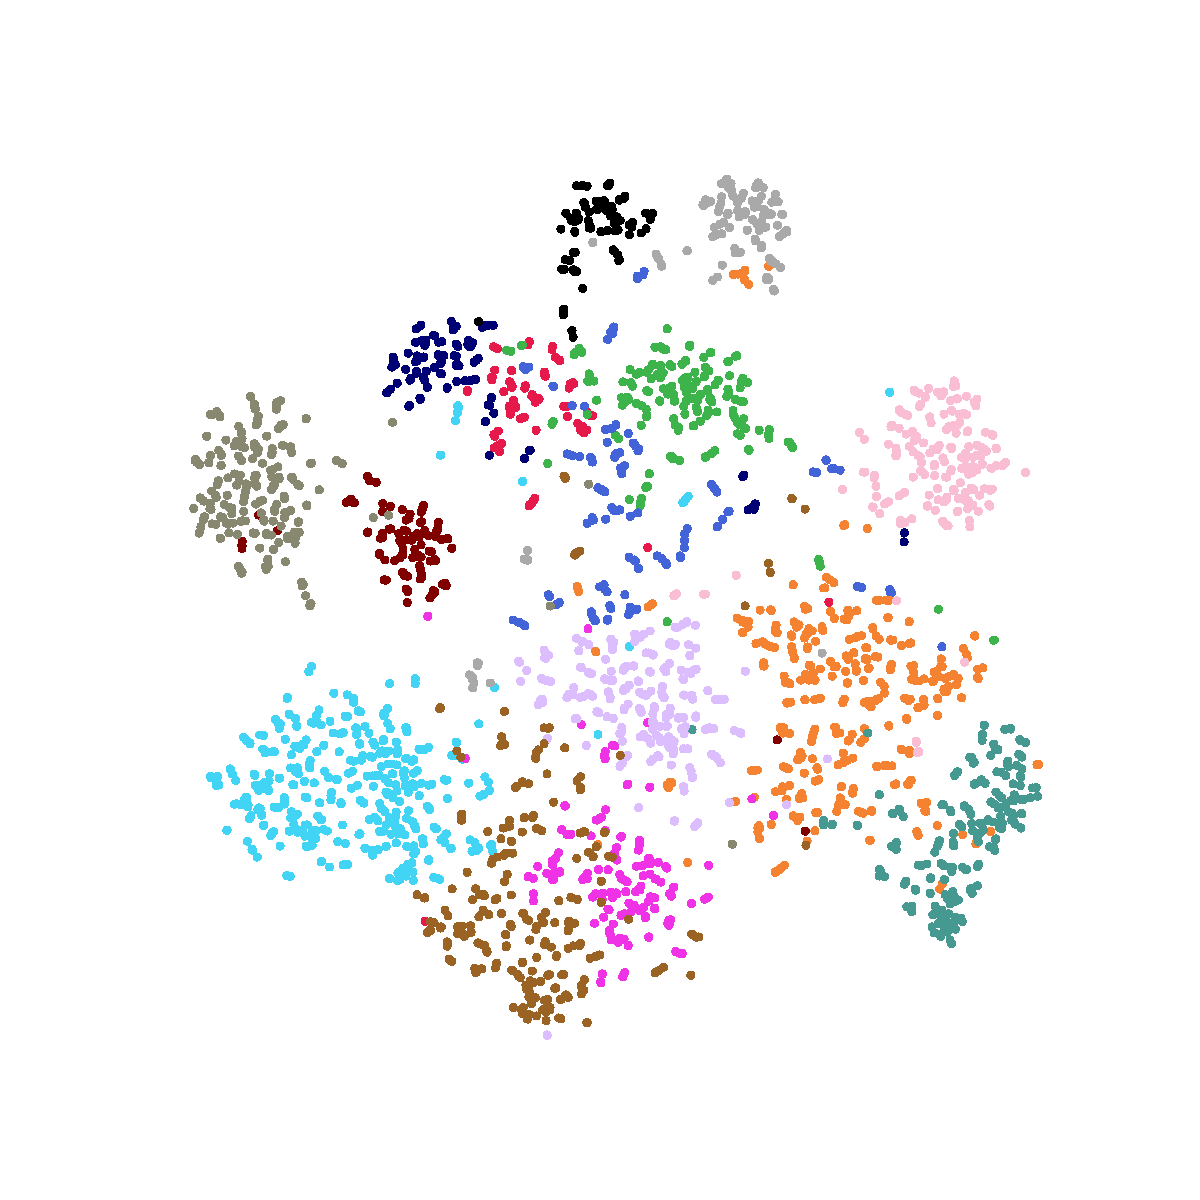
\includegraphics[width=\linewidth]{fig/tsne/point_ladder1.pdf}
        \caption*{\textbf{\#TP}:0.6M \textbf{\#OA}:85.46}
        \caption{PLT (Ours)}
        \label{fig:sub6}
    \end{subfigure}
    \caption{The t-SNE visualizations from the test sets of ScanObjectNN (PB\_T50\_RS) using a pre-trained PointMAE with different fine-tuning strategies. We extract the final classification features from the top linear layer for t-SNE visualizations.}
    \label{fig:tsne}
\end{figure*}